\documentclass[aspectratio=169, 12pt]{beamer}
% packages
\usepackage{multicol}
\usepackage[T2A]{fontenc}
\usepackage[utf8]{inputenc}
\usepackage[english,russian]{babel}
\usepackage{booktabs}
\usepackage{biblatex}
\usepackage{graphicx}
\usepackage{href-ul}
\usepackage{cmap}
\usepackage{svg}

\usepackage{lipsum}

\usepackage{icomma}
\usepackage{amsthm}
\usepackage{graphicx}
\usepackage{amssymb}
\usepackage{amsmath}
\usepackage{graphicx}
\usepackage{color}
%\usepackage{bm}
\usepackage{tabularx}
\usepackage{url}
\usepackage{multirow}
\usepackage{wrapfig}
\usepackage{caption}
\usepackage{subcaption}
\usepackage{algorithm}
\usepackage{algpseudocode}
%% Цвета 
%\usepackage{color}
%\usepackage{colortbl}

% Создаем новую команду для assumptions
\newtheorem{assumption_rus}{Предположение}
\newtheorem{theorem_rus}{Теорема}
\newtheorem{lemma_rus}{Лемма}


%beamer  theme's used to be here :)
%\usetheme{mipt_beamer}
\usetheme{boxes}
\beamertemplatenavigationsymbolsempty
\setbeamertemplate{footline}[page number]
%----------------------------------------------------------------------------------------------------------

%%%
\title[\hbox to 56mm{Feature}]{Методы с предобуславливанием и затуханием весов}
\subtitle{\textcolor{black}{Выпускная квалификационная работа бакалавра}}
\author[М.\,К.~Крейнин]{
    Матвей Вадимович Крейнин\\
    Научный руководитель: к.ф.-м.н. А.\,Н.~Безносиков
}
\institute[МФТИ (НИУ)]{
\small{
    Кафедра интеллектуальных систем ФПМИ МФТИ\\
    Специализация: Интеллектуальный анализ данных\\
    Направление: 03.03.01 Прикладные математика и физика
}}
\date{2024}
%%%


\begin{document}
\maketitle
\begin{frame}{Методы с предобуславливанием и затуханием весов}
    Исследуется сходимость методов оптимизации с предобуславливанием и затуханием весов.
    \begin{block}{Проблема}
        \vspace{-0.15cm}
        Исследование скорости сходимости методов оптимизации с предобуславливанием.
    \end{block}
    \begin{block}{Цель}
        \vspace{-0.15cm}
        Оценить скорость сходимости данных методов и предложить альтернативный вариант добавления регуляризации.
    \end{block}
\end{frame}

\begin{frame}{Постановка задачи}
     \begin{columns}[t]
    \begin{column}{0.48\textwidth}
        \vspace{-0.5cm}
        \begin{block}{Классическое решение}
        \begin{equation}
        \label{eq:general}
            \min_{w \in \mathbb{R}^d} f(w)
        \end{equation} 
        \end{block}
        \textbf{Метод градиентного спуска}
        \begin{equation*}
            w_t = w_{t-1} - \eta \nabla f(w_t).
        \end{equation*}
        \textbf{Метод Ньютона}:
        \begin{equation*}
            w_t = w_{t_-1} - \eta \left( \nabla^2 f(w_{t-1}) \right)^{-1} \nabla f(w_{t-1})
        \end{equation*}
    \end{column}
    \hspace{0.5cm}
    \vrule
    \hspace{0.5cm}
    \begin{column}{0.48\textwidth}
        \vspace{-0.5cm}
        \begin{block}{Метод стохастического градиента}
        \begin{equation*}
            w_{t+1} = w_t - \eta g_t,
        \end{equation*}
        $g_t$ - несмещённый стохастический градиент
        \end{block}
        
        \begin{block}{Методы с предобуславливанием}
        \begin{equation*}
            w_{t+1} = w_t - \eta D_t^{-1}g_t,
        \end{equation*}
        $D_t$ -- матрица предобуславливания.
        \end{block}
    \end{column}
\end{columns}
\end{frame}

\begin{frame}[shrink]{Новая минимизируемая функция}
\begin{equation*}
        \min_{w \in \mathbb{R}^d} F(w) := f(w) + r(w), \text{$r(w)$ это функция регуляризации.}
\end{equation*}


\begin{algorithm}[H]
    \caption{Способы использования предобуславливания с регуляризацией}
    \label{alg:precond}
    
    \begin{algorithmic}
            \Require{$\eta$ $-$ шаг обучения, $f$ $-$ оптимзируемая функция}
            
            \While {$w$ не сойдется}
            \State $t = t+1$
            \State $g_t \gets$ стохастический градиент $f$
            \State $\textcolor{blue}{g_t \gets g_t + \nabla r(w_t)}$ \hfill \textcolor{blue}{обычная регуляризация}
            \State $D_t \gets$ матрица предобуславливания с помощью $g_t$

            \State \textcolor{blue}{$w_t \gets w_{t-1} - \eta \cdot D_t^{-1}g_t $} \hfill \textcolor{blue}{обычная регуляризация}, 
            \State \textcolor{orange}{$w_t \gets w_{t-1} - \eta \cdot D_t^{-1} \left(g_t +\nabla r(w_t) \right)$} \hfill \textcolor{orange}{масштабированное затухание весов}, 
            \State \textcolor{red}{$w_t \gets w_{t-1} - \eta \cdot D_t^{-1} g_t  - \eta \cdot \nabla r(w_t)$} \hfill \textcolor{red}{затухание весов}, 
            \EndWhile
    \end{algorithmic}
\end{algorithm}
\end{frame}

\begin{frame}{Альтернативный взгляд}

Вынесем $D_t^{-1}$ за скобки и получим новый градиент:
\begin{equation*}
    w_{t+1} = w_t - \eta D_t^{-1}(\nabla f(w_t) + D_t \nabla r(w_t))
\end{equation*}
Новая функция регуляризации $\nabla \tilde{r}(w) = D_t \nabla r(w)$.


Задача минимизации, которая решается непосредственно:
\begin{equation*}
\label{F_tilde}
    \min_{w \in \mathbb{R}^d} \tilde{F}(w) := f(w) + \tilde{r}(w)
\end{equation*}
где $\tilde{F}(w)$ изменяется на каждом шаге.
\end{frame}

\begin{frame}{Предположения на функции}

\begin{columns}[t]
    \begin{column}{0.48\textwidth}
        \vspace{-0.5cm}
        \begin{assumption_rus}[Структура регулязитора]
    \label{ass:regstruct}
    Регуляризатор $r$ сепарабелен:
    $$r(w) = \sum_{i=1}^d r_i(w^i),$$
    где $r_i(x) \ge 0$ для $i \in \overline{1, d}$ и $x \in \mathbb{R}$.
\end{assumption_rus}
\begin{assumption_rus}[Сильная выпуклость]
    \label{ass:muconvex}
    $\exists \mu_f : \forall x, y \in \mathbb{R}^d$ выполняется:
    $$
    f(y) \geq f(x) + \langle \nabla f(x), y-x \rangle + \frac{\mu_f}{2} ||x-y||_2^2.
    $$
\end{assumption_rus}
    \end{column}
    \hspace{0.5cm}
    \vrule
    \hspace{0.5cm}
    \begin{column}{0.48\textwidth}
        \vspace{-0.5cm}
\begin{assumption_rus}[Структура матрицы предобуславливания]
    \label{ass:precondstruct}
    Матрица предобуславливания $D_t$ может быть представлена в следующем виде:
     $D_t = \textrm{diag} \left\{ d_t^1 \ldots, d
_t^d \right\}.$
\end{assumption_rus}
\begin{assumption_rus}[Ограниченность предобуславливателя]
\label{ass:preconditioned}
$\exists$ $\alpha, \Gamma \in \mathbb{R} : 0 < \alpha < \Gamma$:
\begin{equation*}
\alpha I \preccurlyeq D_t \preccurlyeq \Gamma I \Leftrightarrow \frac{I}{\Gamma} \preccurlyeq D_t^{-1} \preccurlyeq \frac{I}{\alpha}.
\end{equation*}
\end{assumption_rus}
    \end{column}
\end{columns}


\end{frame}

\begin{frame}{Предположения на функции}
     \begin{columns}[t]
    \begin{column}{0.48\textwidth}
        \vspace{-0.6cm}
        \begin{assumption_rus}[$L$-гладкость]
\label{ass:smoothness}

    Градиент функции $f$ является $L_f$-гладким, $\exists$ $L_f > 0:$ $\forall x, y \in \mathbb{R}^d$,
    	\begin{equation*}
    		f(x) \leq f(y) + \langle \nabla f(y), x-y \rangle + \frac{L_f}{2} \|x - y\|^2.
    	\end{equation*}
     \end{assumption_rus}
     \begin{assumption_rus}[$L$-гладкость]
    Градиент функции $r$ является $L_r$-гладким, $\exists$ $L_r > 0:$ $\forall x, y \in \mathbb{R}^d$,
	\begin{equation*}
		r(x) \leq r(y) + \langle \nabla r(y), x-y \rangle + \frac{L_r}{2} ||x - y||^2.
	\end{equation*}
\end{assumption_rus}
    \end{column}
    \hspace{0.5cm}
    \vrule
    \hspace{0.8cm}
    \begin{column}{0.48\textwidth}
    \vspace{-0.5cm}
        \begin{assumption_rus}[Ограниченность регуляризатора]
\label{ass:regbound}
Регуляризатор ограничен, $\exists$ $\Omega > 0:$ \\ 
$\forall w \in \mathbb{R}^d$ выполняется $ |r(w)| \le \Omega.$
\end{assumption_rus}
\begin{assumption_rus}[Ожидания]
$g_t$ являются несмещенными и имеют ограниченную вариацию на любом шаге, то есть
\begin{equation*}
\mathbb{E}\left[ g_t \right] = \nabla f (w_t), \mathbb{E}\left[ ||g_t - \nabla f||^2 \right] \leq \sigma^2,
\end{equation*}
\label{ass:expectations}
\end{assumption_rus}
    \end{column}
\end{columns}
\end{frame}
\begin{frame}{Леммы}
    \begin{lemma_rus}[Существование $\widetilde{r}$]
\label{lemma:existence}
    Предполагая, что \ref{ass:regstruct}, \ref{ass:precondstruct} выполняются, функция $\widetilde{r}$ существует и имеет следующую форму:
    $$\widetilde{r}_t(w) = \sum_{i=1}^d d_t^i r_i(w_i)$$
\end{lemma_rus}

\begin{lemma_rus}\label{lemma:tildesmoothness}{(L-гладкость $\widetilde{r}$)}
Предполагая, что \ref{ass:regstruct}, \ref{ass:precondstruct}, \ref{ass:smoothness}, \ref{ass:preconditioned} выполняются,
градиент $\widetilde{r}$ является $L_{\tilde{r}}$-непрерывным, 
то есть существует константа  $L_{\tilde{r}} > 0$ такая, что $\forall x, y \in \mathbb{R}^d$,
\begin{equation*}
    		\widetilde{r}_t(x) \leq \widetilde{r}_t(y) + \langle \nabla \widetilde{r}_t(y), x-y \rangle + \frac{L_{\tilde{r}}}{2} ||x - y||^2,
    	\end{equation*}
     и $L_{\tilde{r}} = \Gamma L_r$.
\end{lemma_rus}
\end{frame}

\begin{frame}{Теоремы}
    \begin{theorem_rus} 
    \label{theor:1}
    Предполагая, что \ref{ass:regstruct}, \ref{ass:precondstruct}, \ref{ass:smoothness}, \ref{ass:regbound}, \ref{ass:preconditioned} выполняются, положим ошибку $\varepsilon > 0$ и шаг обучения удовлетворяют условию: $\eta < \frac{2 \alpha}{L_f + \Gamma L_{r}}$.
    Количество итераций, начиная с начальной точки $w_0 \in \mathbb{R}^d$ , $\Delta_0 = \tilde{F}_0(w_0) - f^*$, где $\widetilde{F}_t$ определено в \eqref{F_tilde} и $f^*$ решением задачи \eqref{eq:general}, 
    необходимое для $\varepsilon$-приближения нормы градиента к 0, может быть ограничено количеством шагов    
    \begin{equation*}
      T = \mathcal{O}\left( \frac{\Delta_0 \Gamma}{(\eta - \frac{\tilde{L}\eta^2}{2\alpha}) \left( \varepsilon -\frac{\delta\Gamma}{\eta - \frac{\tilde{L}\eta^2}{2\alpha}}\right)} \right),
\end{equation*}
$\widetilde{L} = L_f + \Gamma L_{r}$ и $\delta=\frac{(1 - \beta)\Gamma^2}{2\alpha}$ выбирается сколь угодно благодаря $\alpha, \beta, \Gamma$. 
\end{theorem_rus}
\end{frame}

\begin{frame}{Теоремы}
    \begin{theorem_rus}
    Преполагая, что \ref{ass:regstruct}, \ref{ass:precondstruct}, \ref{ass:smoothness}, \ref{ass:regbound}, \ref{ass:preconditioned}, \ref{ass:muconvex} выполняются, положим ошибку $\varepsilon > 0$ и шаг обучения удовлетворяют условию: 
    $$
    \eta < \eta_{min} = \min \left\{ \frac{2L_f \Omega_0^2}{\alpha \beta^2}; \frac{\alpha}{4L_f}; \frac{8\mu_f L_f^2 \Omega_0^4}{\alpha^2 \beta^4} + \frac{L_f \Omega_0^2}{\alpha \beta^2} \right\},
    $$ гиперпараметры удовлетворяют условиям: $\lambda < \frac{\alpha \beta^2}{8L_f \Omega_0^2}$, $\beta \geq 1 - \frac{\eta(\mu_f + \lambda)\alpha}{2 \Gamma^2}$. Получаем оценку на необходимое количество шагов для сходимости алгоритма к заданной точности:
    $$T = \mathcal{O} \left(\log\left(\frac{R_0^2 + \frac{8\lambda \Omega_0^2 \Gamma^2}{\alpha^2(\mu_f+\lambda)} \sigma_0^2}{\varepsilon} \right) \frac{4}{\eta_{min} (\mu_f + \lambda)\cdot \min \left\{1; \frac{2\alpha}{\Gamma^2} \right\} } \right)$$
\end{theorem_rus}
\end{frame}

\begin{frame}{AdamW}
    \begin{algorithm}[H]
            \caption{Adam}\label{alg:genAdam}    
            \begin{algorithmic}
            \small{
            \Require{$\eta, \beta_1, \beta_2, \epsilon, f, r$}
            %\State $m_0 = 0$ -- 1-st moment vector
            %\State$v_0 = 0$ -- 2-nd moment vector
            \While {$\theta$ not converged}
            \State $t = t+1$
            \State $g_t = \nabla f(w_{t-1}) + $ \textcolor{blue}{$\nabla r(w_{t-1})$}\hfill \textcolor{blue}{AdamL2}
            \State $m_t = \beta_1 \cdot m_{t-1} + (1 - \beta_1) \cdot g_t$
            \State $v_t = \beta_2 \cdot v_{t-1} + (1 - \beta_2) \cdot g_t^2$
            \State $\hat{m_t} = \frac{m_t}{1-\beta_1^t} +$ \textcolor{orange}{$\nabla r(w_{t-1})$} \hfill \textcolor{orange}{AdamWH}
            \State $\hat{v_t} = \frac{v_t}{1-\beta_2^t}$ 
            \State $w_t = w_{t-1} - \eta \cdot \frac{\hat{m_t}}{\sqrt{v_t} + \epsilon} - $ \textcolor{red}{$\eta \nabla r(w_{t-1})$ } \hfill \textcolor{red}{AdamW}
            \EndWhile
            }
\end{algorithmic}
\end{algorithm}
\end{frame}

\begin{frame}{Эксперименты}
\begin{figure}[H]
\begin{minipage}[h]{0.49\linewidth}
\centering
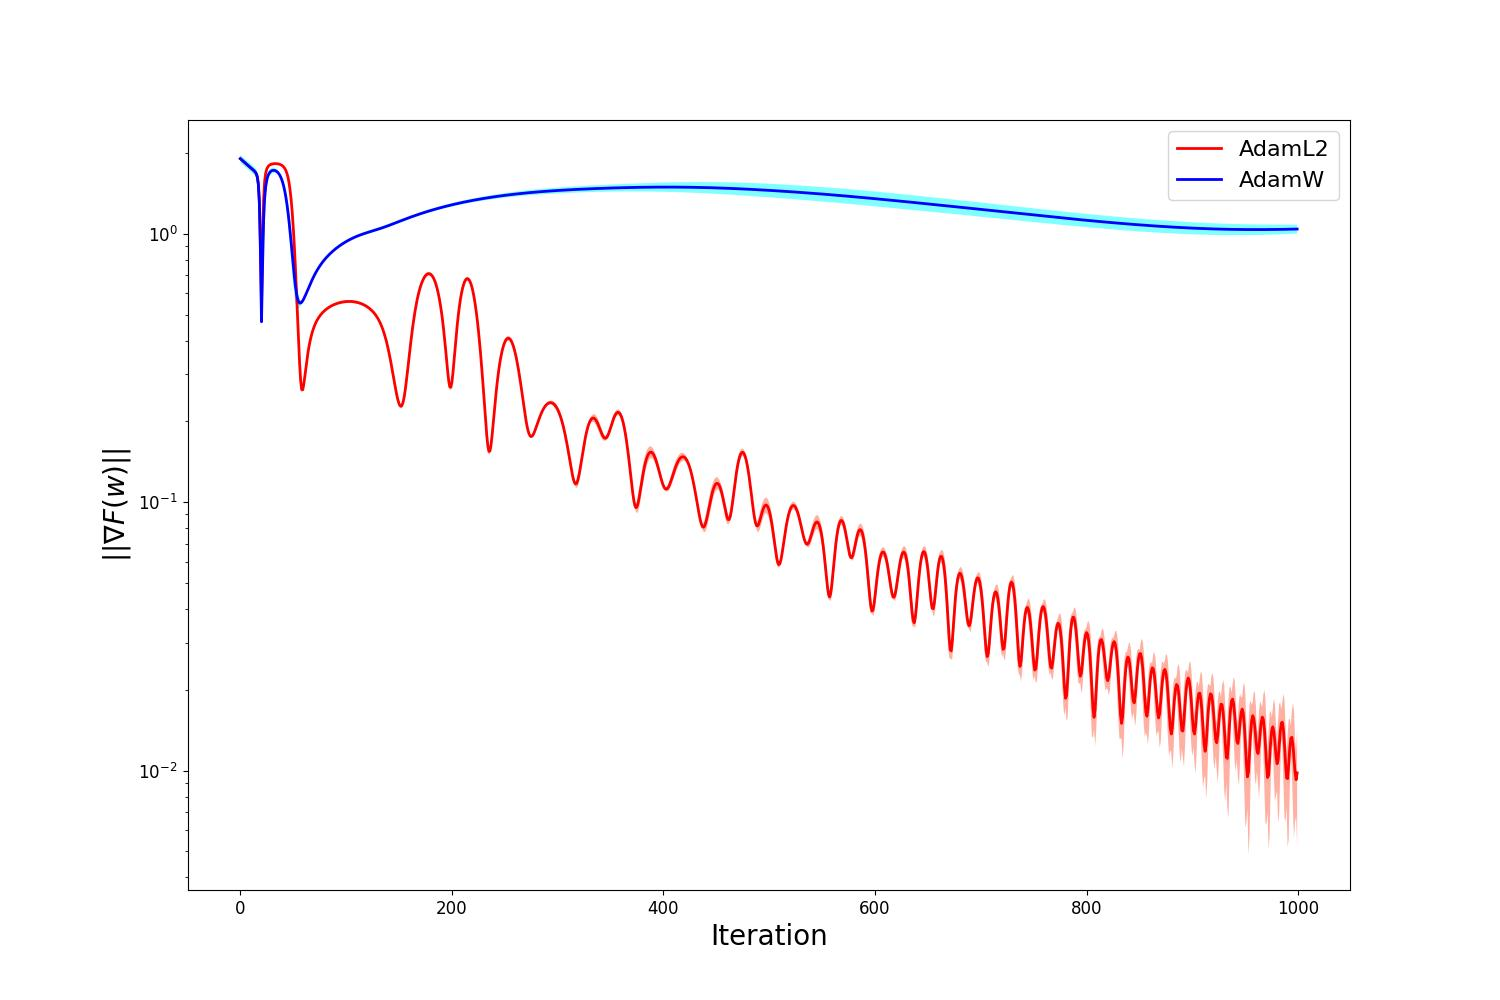
\includegraphics[width=\linewidth]{fig1.jpg}
\caption{Adam and AdamW по критерию, $||\nabla F(w)|| = ||\nabla f(w) + \nabla r(w)||$}
\label{fig:adams_errors}
\end{minipage}
\hfill
\begin{minipage}[h]{0.49\linewidth}
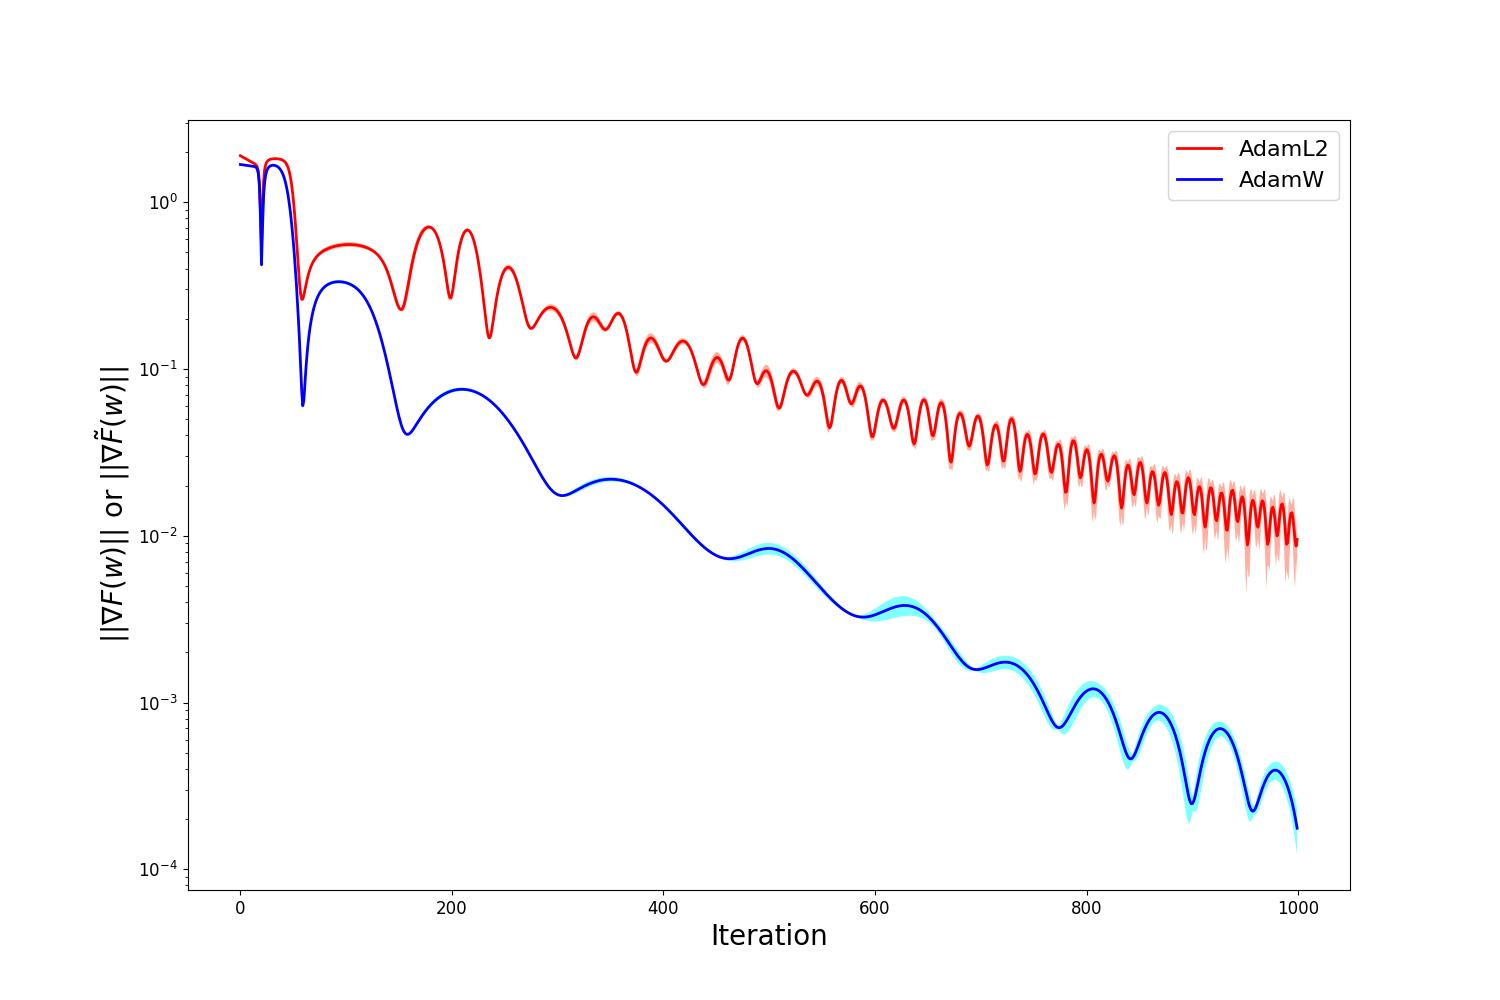
\includegraphics[width=\linewidth]{fig2.jpg}
\caption{Adam and AdamW по критерию, $||\nabla \tilde{F}(w)|| = ||\nabla f(w) + \nabla \tilde{r}(w)||$}
\label{fig:adams_special_errors}
\end{minipage}
\end{figure}
\end{frame}

\begin{frame}{На защиту выносится}
    \begin{enumerate}
        \item Исследована теоретическая сходимость методов.
        \item Новый метод добавления регуляризатора в методы с предобуславливанием.
        \item Две леммы о существовании, структуре и гладкости измененного регуляризатора.
        \item Теорема о сходимости методов с предобуславливанием и затуханием весов по норме градиента.
        \item Теорема о сходимости методов с предобуславливанием и затуханием весов по аргументу.
    \end{enumerate}
\end{frame}


\end{document}